%
% wavelets.tex -- Wavelets auf Graphen
%
% (c) 2020 Prof Dr Andreas Müller, Hochschule Rapperswil
%
\section{Wavelets auf Graphen
\label{buch:section:wavelets-auf-graphen}}
\rhead{Wavelets auf Graphen}
In Abschnitt~\ref{buch:subsection:standardbasis-und-eigenbasis} wurde
gezeigt dass die Standardbasis den Zusammenhang zwischen den einzelnen
Teilen des Graphen völlig ignoriert, während die Eigenbasis Wellen
beschreibt, die mit vergleichbarer Amplitude sich über den ganzen
Graphen erstrecken.
Die Eigenbasis unterdrückt also die ``Individualität'' der einzelnen
Knoten fast vollständig.

Wenn man einen Standardbasisvektor in einem Knoten $i$
als Anfangstemperaturverteilung verwendet, erwartet man eine Lösung,
die für kleine Zeiten $t$ die Energie immer in der Nähe des Knotens $i$
konzentriert hat.
Weder die Standardbasis noch die Eigenbasis haben diese Eigenschaft.

\subsection{Vergleich mit der Wärmeleitung auf $\mathbb{R}$}
Ein ähnliches Phänomen findet man bei der Wärmeausbreitung gemäss
der partiellen Differentialgleichung
\[
\frac{\partial T}{\partial t} = -\kappa \frac{\partial^2 T}{\partial x^2}.
\]
Die von Fourier erfundene Methode, die Fourier-Theorie, verwendet die
Funktionen $e^{ik x}$, die Eigenvektoren der zweiten Ableitung
$\partial^2/\partial x^2$ sind.
Diese haben das gleiche Problem, der Betrag von $e^{ikx}$ ist $1$, die
Entfernung von einem Punkt spielt überhaupt keine Rolle.
Die Funktion
\[
F(x,t)
=
\frac{1}{\sqrt{4\pi\kappa t}}e^{-x^2/4\kappa t}
\]
ist eine Lösung der Wärmeleitungsgleichung mit einem Maximum an
der Stelle $0$.
Sie heisst die Fundamentallösung der Wärmeleitungsgleichung.
Durch Überlagerung von Translaten in eine Funktion
\begin{equation}
f(x,t)
=
\int_{-\infty}^\infty f(\xi) F(x-\xi,t)\,d\xi
\label{buch:graphen:eqn:fundamentalueberlagerung}
\end{equation}
kann man die allgemeine Lösung aus Fundamentallösungen zusammensetzen.
Die Fundamentallösungen $f(x-\xi,t)$ sind für kleine Zeiten immer noch
deutlich in einer Umgebung von $\xi$ konzentriert.

% XXX Ausbreitung der Fundamentallösung illustrieren
\begin{figure}
\centering
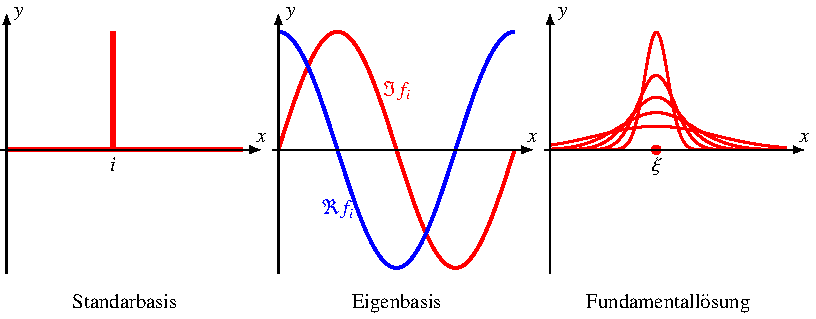
\includegraphics{chapters/70-graphen/images/fundamental.pdf}
\caption{Vergleich der verschiedenen Funktionenfamilien, mit denen
Lösungenfunktionen durch Linearkombination erzeugt werden können.
In der Standarbasis (links) ist es am einfachsten, die Funktionswerte
abzulesen, in der Eigenbasis (Mitte) kann die zeitliche Entwicklung
besonders leicht berechnet werden.
Dazuwischen liegen die Fundamentallösungen (rechts), die eine einigermassen
übersichtliche Zeitentwicklung haben, die Berechnung der Temperatur an 
einer Stelle $x$ zur Zeit $t$ ist aber erst durch das Integral
\eqref{buch:graphen:eqn:fundamentalueberlagerung} gegeben.
\label{buch:graphen:fig:fundamental}}
\end{figure}

\subsection{Fundamentallösungen auf einem Graphen}
Die Wärmeleitungsgleichung auf einem Graphen kann für einen
Standardbasisvektor mit Hilfe der
Lösungsformel~\eqref{buch:graphen:eqn:eigloesung}
gefunden werden.
Aus physikalischen Gründen ist aber offensichtlich, dass die
Wärmeenergie Fundamentallösungen $F_i(t)$ für kurze Zeiten $t$
in der Nähe des Knoten $i$ konzentriert ist.
Dies ist aber aus der expliziten Formel
\begin{equation}
F_i(t)
=
\sum_{j=1}^n \langle f_j,e_i\rangle e^{-\kappa \lambda_i t} f_j
=
\sum_{j=1}^n \overline{f}_{ji} e^{-\kappa \lambda_i t},
\label{buch:graphen:eqn:fundamentalgraph}
\end{equation}
nicht unmittelbar erkennbar.

Man kann aber aus~\eqref{buch:graphen:eqn:fundamentalgraph} ablesen,
dass für zunehmende Zeit die hohen Frequenzen sehr schnell gedämpft
werden.
Die hohen Frequenzen erzeugen also den scharfen Peak für Zeiten nahe
beim Knoten $i$, die zu kleineren $\lambda_i$ beschreiben die Ausbreitung
über grössere Distanzen.
Die Fundamentallösung interpoliert also in einem gewissen Sinne zwischen
den Extremen der Standardbasis und der Eigenbasis.
Die ``Interpolation'' geht von der Differentialgleichung aus,
sie ist nicht einfach nur ein Filter, der die verschiedenen Frequenzen
auf die gleiche Art bearbeitet.

Gesucht ist eine Methode, eine Familie von Vektoren zu finden,
aus der sich alle Vektoren linear kombinieren lassen, in der aber
auch auf die für die Anwendung interessante Längenskala angepasste
Funktionen gefunden werden können.

\subsection{Wavelets auf einem Graphen}
Die Fourier-Theorie analysiert Funktionen nach Frequenzen, wobei die 
zeitliche Position von interessanten Stellen der Funktion in der Phase
der einzelnen Komponenten verschwindet.
Die Lokalisierung geht also für viele praktische Zwecke verloren.
Umgekehrt haben einzelne Ereignisse wie eine $\delta$-Funktion keine
charakteristische Frequenz, sie sind daher im Frequenzraum überhaupt 
nicht lokalisierbar.
Die Darstellung im Frequenzraum und in der Zeit sind also extreme
Darstellungen, entweder Frequenzlokalisierung oder zeitliche Lokalisierung
ermöglichen, sich aber gegenseitig ausschliessen.

\subsubsection{Dilatation}
Eine Wavelet-Basis für die $L^2$-Funktionen auf $\mathbb{R}$ erlaubt
eine Funktion auf $\mathbb{R}$ auf eine Art zu analysieren, die eine
ungenaue zeitliche Lokalisierung bei entsprechend ungenauer
Frequenzbestimmung ermöglicht.
Ausserdem entstehen die Wavelet-Funktionen aus einer einzigen Funktion
$\psi(t)$ durch Translation um $b$ und Dilatation mit dem Faktor $a$:
\[
\psi_{a,b}(t)
=
\frac{1}{\sqrt{|a|}} \psi\biggl(\frac{t-b}a\biggr)
=
T_bD_a\psi(t)
\]
in der Notation von \cite{buch:mathsem-wavelets}.
Auf einem Graphen ist so eine Konstruktion grundsätzlich nicht möglich,
da es darauf weder eine Translations- noch eine Streckungsoperation gibt.

In der Theorie der diskreten Wavelet-Transformation ist es üblich, sich
auf Zweierpotenzen als Streckungsfaktoren zu beschränken.
Ein Gitter wird dadurch auf sich selbst abgebildet, aber auf einem
Graphen gibt es keine Rechtfertigung für diese spezielle Wahl von
Streckungsfaktoren mehr.
Es stellt sich daher die Frage, ob man für eine beliebige Menge
\(
T= \{ t_1,t_2,\dots\} \}
\)
von Streckungsfaktoren eine Familie von Funktionen $\chi_j$ zu finden
derart, dass man sich die $\chi_j$ in einem gewissen Sinn als aus
$\chi_0$ durch Dilatation entstanden vorstellen kann.

Die Dilatation kann natürlich nicht von einer echten
Dilatation im Ortsraum herstammen, aber man kann wenigstens versuchen, die
Dilatation im Frequenzraum nachzubilden.
Für Funktionen in $L^2(\mathbb{R})$ entspricht die Dilatation mit dem
Faktor $a$ im Ortsraum der Dilatation mit dem Faktor $1/a$ im Frequenzraum:
\[
\widehat{D_af}(\omega) = D_{1/a}\hat{f}(\omega).
\]
\cite[Satz~3.14]{buch:mathsem-wavelets}.
Es bleibt aber das Problem, dass sich auch die Skalierung im Frequenzraum
nicht durchführen lässt, da auch das Frequenzspektrum des Graphen nur eine
Menge von reellen Zahlen ohne innere algebraische Struktur ist.

\subsubsection{Mutterwavelets}
\begin{figure}
\centering
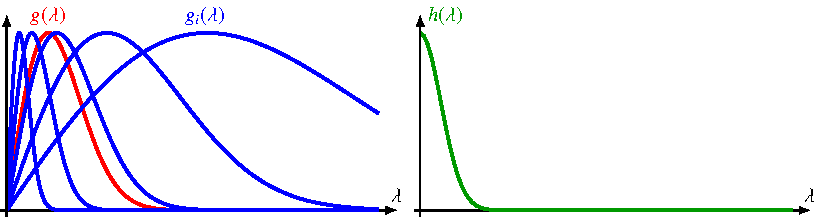
\includegraphics{chapters/70-graphen/images/gh.pdf}
\caption{Lokalisierungsfunktion $g(\lambda)$ für die Dilatation (links).
Die Dilatierten Funktionen $g_i=\tilde{D}_{1/a_i}g$ lokalisieren
die Frequenzen jeweils um die Frequenzen $a_i$ im Frequenzraum.
Der Konstante Vektor ist vollständig delokalisiert, die Funktion $h$
in der rechten Abbildung entfernt die hohen Frequenzen und liefert Funktionen,
die in der Umgebung eines Knotens wie die Konstante Funktion aussehen.
\label{buch:graphs:fig:lokalisierung}}
\end{figure}
Das Mutter-Wavelet einer Wavelet-Analyse zeichnet definiert, in welchem Mass
sich Funktionen im Orts- und im Frequenzraum lokalisieren lassen.
Die Standardbasis der Funktionen auf einem Graphen repräsentieren die
perfekte örtliche Lokalisierung, Eigenbasis der Laplace-Matrix $L$ repräsentiert
die perfekte Lokalisierung im Frequenzraum.
Sei $g(\lambda)\ge 0$ eine Funktion im Frequenzraum, die für  $\lambda\to0$ und
$\lambda\to\infty$ rasch abfällt mit einem Maximum irgendwo dazwischen
(Abbildung~\ref{buch:graphs:fig:lokalisierung}).
Sie kann als eine Lokalisierungsfunktion im Frequenzraum betrachtet werden.

Die Matrix $g(L)$ bildet entfernt aus einer Funktion die ganz hohen und 
die ganz tiefen Frequenz, lokalisiert also die Funktionen im Frequenzraum.
Die Standardbasisvektoren werden dabei zu Funktionen, die nicht mehr nur
auf einem Knoten von $0$ verschieden sind, aber immer noch einigermassen
auf dem Graphen lokalisiert sind.
Natürlich sind vor allem die Werte auf den Eigenwerten
$\lambda_0 < \lambda_1\le \dots\le \lambda_n$ der Laplace-Matrix
von Interesse.

Die Matrix $g(L)$ kann mit Hilfe der Spektraltheorie berechnet werden,
was im vorliegenden Fall naheliegend ist, weil ja die Eigenvektoren von
der Laplace-Matrix bereits bekannt sind.
Die Matrix $\chi^t$ bildet die Standardbasisvektoren in die
Eigenbasis-Vektoren ab, also in eine Zerlegung im Frequenzraum ab,
$\chi$ vermittelt die Umkehrabbildung.
Mit der Spektraltheorie findet man für die Abbildung $g(L)$ die Matrix
\begin{equation}
g(L)
=
\chi
\begin{pmatrix}
g(\lambda_0)&0&\dots&0\\
0&g(\lambda_1)&\dots&0\\
\vdots&\vdots&\ddots&\vdots\\
0&0&\dots&g(\lambda_n)
\end{pmatrix}
\chi^t.
\label{buch:graphen:eqn:mutterwavelet}
\end{equation}

\subsubsection{Dilatation}
Die Dilatation um $a$ im Ortsraum wird zu einer Dilatation um $1/a$ im
Frequenzraum.
Statt also nach einer echten Dilatation der Spaltenvektoren in $g(L)$
zu suchen, kann man sich darauf verlegen, Funktionen zu finden, deren
Spektrum von einer Funktionen lokalisiert worden ist, die eine Dilatation
von $g$ ist.
Man wählt daher eine ansteigende Folge $A=(a_1,\dots)$ von Streckungsfaktoren
und betrachtet anstelle von $g$ die dilatierten Funktionen
$g_i=\tilde{D}_{1/a_i}g$.
Die zugehörigen Wavelet-Funktionen auf dem Graphen können wieder mit
der Formel~\eqref{buch:graphen:eqn:mutterwavelet} berechnet werden,
man erhält
\begin{equation}
\tilde{D}_{1/a_i}g(L)
=
g_i(L)
=
\chi
\begin{pmatrix}
g(a_i\lambda_0)&0&\dots&0\\
0&g(a_i\lambda_1)&\dots&0\\
\vdots&\vdots&\ddots&\vdots\\
0&0&\dots&g(a_i\lambda_n)
\end{pmatrix}
\chi^t .
\end{equation}
Die Spalten von $g_i(L)$ bilden wieder eine Menge von Funktionen, die
eine gemäss $g_i$ lokalisiertes Spektrum haben.

\subsubsection{Vater-Wavelet}
Wegen $g(0)=0$ wird die konstante Funktion, die Eigenvektor zum Eigenwert
$\lambda_0=0$ ist, von den Abbildungen $g_i(L)$ auf $0$ abgebildet.
Andererseits ist diese Funktion nicht lokalisiert, man möchte Sie also
für die Analyse nicht unbedingt verwenden.
Man wählt daher eine Funktion $h(\lambda)$ mit $h(0)=1$ so, dass
für $\lambda\to \infty$ der Wert $h(\lambda)$ genügend rasch gegen $0$
geht.
Die Matrix $h(L)$ bildet daher den konstanten Vektor nicht auf $0$ ab,
sondern lokalisiert ihn im Ortsraum.
Wir erhalten daher in den Spalten von $h(L)$ Vektoren, die um die
einzelnen Knoten lokalisiert sind.

\subsubsection{Rekonstruktion}
Die Operatoren $h(L)$ und $g_i(L)$ erzeugen analysieren eine Funktion
nach den verschiedenen Frequenzen mit den Skalierungsfaktoren $a_i$,
aber die Rekonstruktion ist noch nicht klar.
Diese wäre einfacher, wenn die Operatoren zusammen die identische
Abbildung ergäben, wenn also
\[
h(L) + \sum_{i}g_i(L)=I
\]
gelten würde.
Nach der Spektraltheorie gilt das nur, wenn für alle Eigenwerte
$\lambda_k$, $k=1,\dots,n$
\[
h(\lambda_k) + \sum_ig(a_i\lambda_k)=1
\]
gilt.
Für beleibige Funktionen $g$ und $h$ kann man nicht davon ausgehen,
aber man kann erwarten.
Man muss daher zusätzlich verlangen, dass
\[
h(\lambda_k) + \sum_{i} g(a_i\lambda_k) > 0
\]
ist für alle Eigenwerte $\lambda_k$.

\subsubsection{Frame}
Die Menge von Vektoren, die in der vorangegangenen Konstruktion gefunden
wurden, ist zu gross, um eine Basis zu sein.
Vektoren lassen sich darin auf verschiedene Art darstellen.
Wir verlangen aber auch keine eindeutige Darstellung, nur eine 
Darstellung, in der wir die ``dominierenden'' Komponenten in jeder
Frequenzskala identifizieren können.

\begin{definition}
\label{buch:graphen:def:frame}
Ein Frame des Vektorraumes $\mathbb{R}^n$ ist eine Menge
$F=\{e_k\;|\; k=1,\dots,N\}$ von Vektoren mit der Eigenschaft
\begin{equation}
A\|v\|^2
\le
\sum_{k=1}^N  |\langle v,e_k\rangle|^2
\le
B\|v\|^2
\label{buch:graphen:eqn:frame}
\end{equation}
Die Zahlen $A$  und $B$ heissen die {\em Frame-Konstanten} des Frames.
\end{definition}

Die oben gefundenen Vektoren, die Spalten Vektoren von $h(L)$ und $g_i(L)$
bilden daher ein Frame.
Die Frame-Konstanten kann man unmittelbar ausrechnen.
Der mittlere Term von \eqref{buch:graphen:eqn:frame} ist 
\[
\|h(L) v\|^2
+
\sum_{i} \|g_i(L)v\|^2,
\]
die durch die Funktion
\[
f(\lambda)
=
h(\lambda)^2 + \sum_i g_i(\lambda)^2
\]
abgeschätzt werden kann.
Die Frame-Konstanten sind daher
\begin{align*}
A&=\min_{k} f(\lambda_k)
&
&\text{und}&
B&=\max_{k} f(\lambda_k).
\end{align*}
Die Konstruktion hat also ein Frame für die Funktionen auf dem Graphen
etabliert, die viele Eigenschaften einer Multiskalenanalyse in diese
wesentlich weniger symmetrische Situation rettet.




